\section{Evaluation}
In this section we present the fault model for the sensors. We further evaluate the failure rates caused due to the faults in the sensor. We address the following research questions:
\begin{enumerate}
	\item \textbf{RQ1}
	What all types of faults can exist in advanced and core sensors of Autonomous vehicles such as the optical sensor.?
	\item \textbf{RQ2}
	What faults do we consider for the autonomous driving systems?
	\item \textbf{RQ3}
	What subset of the above faults cause the most amount of system damage i.e system failure?
	\item \textbf{RQ3}
	What is the failure rate of the faults causing the most amount of damage?
	\item \textbf{RQ5}
	What mitigation strategies can we use for preventing those failure rates due to the particular sensor faults in Autonomous vehicles?
\end{enumerate}
\vskip 0.2in
We answer the above research questions. 
\vskip 0.2in
\textbf{RQ1: What all types of faults exist in advance and core sensors in an autonomous vehicle.}

Though there have been lot of studies which look at the individual sensors. These studies also performed an indepth analysis of the faults which can be present in a sensors such as high-powered camera \cite{5530865}, \cite{inproceedings}. However, none of the previous work categorizes the fault model into hardware faults and image faults as shown in fig. 2. We not only constructed a fault model for the high-powered sensors, but we chose the faults which are most likely to occur in case of a self driving car. The previous work by Bresolin et al. \cite{inproceedings} performs a fault diagnosis of hybrid systems. However, their fault model is limited as they only consider the hardware faults. 

We chose to start our work with optical sensors because of many reasons. Due to the unstable nature of LIDARs a lot of industrial focus is being shifted towards cameras. A recent work says that soon cheap cameras would replace LIDARs\cite{cheapcamera}. Hence to visualize a 3D world a setup can be constructed using a pair of cameras. In order to do so, it becomes an absolute necessity to understand the faults which can be a part of high-powered cameras as well as low powered cameras. 

As shown in Fig. 2 we consider hardware faults and the weather faults. The two major categories we consider in our system are the image noise and the occlusions. Image noise is the random variation of brightness or color information in images.
The effects of image noises are diverse and can vary from causing minimal damage to the image to
a level which makes it difficult to determine the subject in the image. The different types of image noises can occur due to heating up of the camera and the internal circuits. The image noise can also occur due to the different temperature effects. Though there are many existing filter to mitigate the noises, our work is to understand which types of noises despite the numerous filters present cause failure of the system. 

The second types of data faults which we explore are the occlusions. Occlusion means that there is something we want to see, but can't due to some property of our sensor setup or some event. The way of dealing with occlusions varies depending on the way it was caused. If we are developing a system which tracks objects (people, cars, ...) then occlusion occurs if an object you are tracking is hidden (occluded) by another object. Like two persons walking past each other, or a car that drives under a bridge. The problem in this case is what we do when an object disappears and reappears again.

\textbf{RQ2: What faults do we consider for the autonomous driving systems and why?}

In order to validate our results and understand we limit our experimentation model. Based on our judgment and understanding, we find experimenting with data faults more compelling as compared to hardware faults. Our reason are well-justified and we will validate them in the next set of RQs.

\subsection{Limitations of CARLA}
The degree to which CARLA models the real world autonomous driving systems and their interaction with the environment, is dependent on the simulation parameters and driving agents used for controlling the ADS. In real world autonomous driving systems an array of sensors is used, which captures a representation of the environment. This captured data is used by the controller to make driving decisions. CARLA provides the capability to simulate important sensors like cameras and LIDARs but some important sensors like Radar can't be simulated. Moreover the developed driving agents do not incorporate all the sensors available in CARLA. For example, the three driving agents studied by Dosovitskiy et al.~\cite{Dosovitskiy17} do not use LIDAR and rely only on camera output to take driving decisions. Using only camera sensors is not a realistic modeling of real world driving systems. 

There are no open source driving agents currently available that use sensors other than camera so in our study the driving agent we chose also uses only camera sensors. As our focus is on faults in camera sensors, this provides us good insight into reliability of ADS due to these faults. Presence of other sensor in the system may lead to masking of these due to other sensors, which is a more realistic representation of a real world system. Studying the effect sensor faults in presence of other sensors, is the next logical step after studying the reliability of ADS due to individual sensor faults.  
CARLA helped us simulate the optical sensors, in order to understand the failure rates due to image noises and occlusions. We look into different types of occlusions as shows in Fig 2. We test for different noises such as Gaussian noise, salt and pepper noise, speckle noise and Poisson noise. The different types of image noises represent different types of probabilistic faults in an image. For example Gaussian noise distributes the noise uniformly across the entire image. Every image noise has a different probabilistic model. Hence, according to Goodfellow et al. \cite{2014arXiv1412.6572G} we can see that sometimes introducing noise can fool the neural network by giving better results than before. 

We try to understand if all image noises indeed cause the failure of the system. Hence we focus our experimentations in understanding image noise and occlusions.

\textbf{RQ3: What subset of the above faults cause the most amount of system damage i.e system failure?}

Figure~\ref{fig:success_rate} shows the success rate of exhaustive fault injection due to different type of injected faults. It can be seen that hardware faults which are represented as bit flips in do not cause any failure.

\begin{figure}
	\vspace{-0.5em}
	\centering
	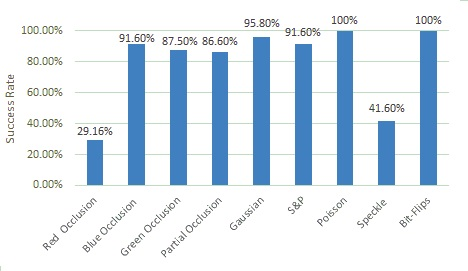
\includegraphics[scale=0.7]{success_rate}
	\vspace{-0.5em}
	\caption{Percentage of trials in which ADS was able to complete specified goals in presence of faults.}
	\label{fig:success_rate}
	\vspace{-1.5em}
\end{figure}

\begin{figure}  
	\vspace{1.0em}
	\centering
	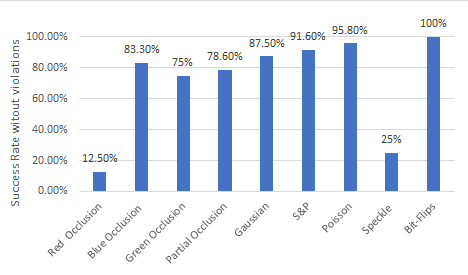
\includegraphics[scale=0.7]{no_violations}
	\vspace{-0.5em}
	\caption{Percentage of trials in which ADS was able to complete specified goals, in presence of faults, without committing any traffic violations.}
	\label{fig:no_violations}
	\vspace{-1.5em}
\end{figure}





